%!TEX TX-program = xelatex

\documentclass[8pt]{article}
\usepackage{allan-eason}

\usetikzlibrary{positioning}
\usetikzlibrary{svg.path}

\graphicspath{ {./images/} }

\newcommand{\Date}{220421}
\newcommand{\Test}{阶段测试}

\newcommand{\Author}{Eason S.}
\newcommand{\Title}{\textcolor{allandarkblue}{\Date}\ \textcolor{allancyan}{\Test}\ 题目选解}

\author{\Author}
\title{\Title}
\date{}

\geometry{a4paper, scale=0.8}

\lhead{\Title}

\begin{document}

	\maketitle

	\section{填空题}
		\defword{1.} 若扇形的圆心角为\(30\degree\), 半径为\(1\), 则扇形的面积为\answord{\(\dfrac{\pi}{12}\)}.

		\answord{解析.} 扇形的面积公式.
		~\\

		\defword{2.} 在\(\triangle ABC\)中, 若\(c = 10\sqrt{2}\), \(C = 60\degree\), \(a = \dfrac{20\sqrt{3}}{3}\), 则\(A = \ansmath{45\degree}\).

		\answord{解析.} 解三角形 (正弦定理).
		~\\

		\defword{3.} 已知\(\tan \theta = \sqrt{2}\), 则\(\sin \left(\dfrac{\pi}{2} + 2\theta\right) = \ansmath{-\dfrac{1}{3}}\).

		\answord{解析.} 三角变换 (诱导公式, 正切半角公式).
		~\\

		\defword{4.} 已知向量\(\vec{a}, \vec{b}\)夹角为\(45\degree\), 且\(\abs{\vec{a}} = 1\), \(\abs{\vec{b}} = 3\sqrt{2}\), 则\(\vec{a} \cdot \left(4\vec{a} - \vec{b}\right) = \ansmath{1}\).

		\answord{解析.} 向量的基本运算.
		~\\

		\defword{5.} 已知\(\tan \theta = \dfrac{1}{2}\), 则\(\sin 2\theta - 2\cos^2 \theta = \ansmath{-\dfrac{4}{5}}\).

		\answord{解析.} 三角变换 (正切半角公式).
		~\\

		\defword{6.} 已知函数\(f(x) = \sin \left(3x + \varphi\right) \left(-\dfrac{\pi}{2} < \varphi < \dfrac{\pi}{2}\right)\)的图像关于直线\(x = \dfrac{\pi}{4}\)对称, 则\(\varphi = \ansmath{-\dfrac{\pi}{4}}\).

		\answord{解析.} 三角函数 (图像).
		~\\

		\defword{7.} 如图,海上某货轮在\(A\)处看灯塔\(B\)在货轮的北偏东\(75\degree\), 距离为\(12\sqrt{6}\)海里; 在\(A\)处看灯塔\(C\)在货轮的北偏西\(30\degree\),距离为\(8\sqrt{3}\)海里, 货轮向正北由\(A\)处行驶到\(D\)处时,若灯塔\(B\)在方位角\(120\degree\)的方向上, 则灯塔\(C\)与\(D\)处之间的距离为\answord{\(8\sqrt{3}\)}海里.

		\[
			\begin{tikzpicture}[scale = 0.25]
				\draw[black, ->] (0, 0)--(0, 10) node[above] {北};
				\draw[black] (0, 0)--(-3, 5)--(0, 6)--(5, 3)--(0, 0) node at (-3, 5) [anchor = east] {\(C\)} node at (0, 0) [anchor = north]{\(A\)} node at (5, 3) [anchor = west] {\(B\)} node at (0, 6) [anchor = south east] {\(D\)};
			\end{tikzpicture}
		\]

		\answord{解析.} 解三角形应用题.
		~\\

		\defword{8.} 已知\(\alpha \in \left(0, \dfrac{\pi}{2}\right)\), \(\beta \in \left(-\pi. -\dfrac{\pi}{2}\right)\), \(\sin \alpha = \dfrac{7\sqrt{2}}{10}\), \(\cos \beta = - \dfrac{2\sqrt{5}}{5}\), 则\(\alpha + 2\beta = \ansmath{-\dfrac{5}{4}\pi}\).

		\answord{解析.} 基本三角方程.
		~\\

		\defword{9.} 关于\(x\)的方程\(\cos^2 x + \sin x - a = 0\)有实数解, 则实数\(a\)的取值范围是\answord{\(\left[-1, \dfrac{5}{4}\right]\)}.

		\answord{解析.} 三角方程, 二次函数.

		\(h(x) \ddef \cos^2 x + \sin x, f(x) \ddef -x^2 + x + 1, g(x) \ddef \sin x,\) 有 \(h(x) = f(g(x))\), \(\displaystyle a \in \left\{h(x) | x \in \RR\right\} = \left\{f(x) | x \in [-1, 1]\right\}\)绘制\(f(x)\)在\([-1, 1]\)上的图像.

		\[
			\begin{tikzpicture}[scale = 1]
				\draw[black, ->] (-1.5, 0)--(1.5, 0) node[below] {\(x\)};
				\draw[black, ->] (0, -2)--(0, 2) node[right] {\(y\)};
				\draw[black, domain = -1 : 1, samples = 2000] plot(\x, {-\x * \x + \x + 1});
			\end{tikzpicture}
		\]

		有\(\ansmath{a \in} \left\{f(x) | x \in [-1, 1]\right\} = \left[f(-1), f\left(\dfrac{1}{2}\right)\right] = \ansmath{\left[-1, \dfrac{5}{4}\right]}\).

		~\\

		\defword{10.} 在\(\triangle ABC\)中, 若\(\cos B = \dfrac{\sqrt{2}}{2}\), 则\(\left(\tan^2 A - 3\right) \sin 2C\)的最小值为\answord{\(-6 + 4\sqrt{2}\)}.

		\answord{解析.} 基本三角方程, 三角变换, 基本不等式.

		\(\cos B = \dfrac{\sqrt{2}}{2} \Rightarrow B = \dfrac{\pi}{4}\),

		\begin{align*}
			\left(\tan^2 A - 3\right)\sin 2C &= \left(\tan^2 A - 3\right) \sin \left[2 \left(\pi - A - B\right)\right] \\
			                                 &= \frac{\sin^2 A - 3\cos^2 A}{\cos^2 A} \sin \left(2\pi - \dfrac{\pi}{2} - 2A\right)\\
			                                 &= \frac{\sin^2 A - 3\cos^2 A}{\cos^2 A} \left(-\cos 2A\right)\\
			                                 &= \frac{\frac{1 - \cos 2A}{2} - 3 \cdot \frac{1 + \cos 2A}{2}}{\frac{1 + \cos 2A}{2}} \left(- \cos 2A\right)\\
			                                 &= \frac{\frac{1 - \cos 2A - 3 - 3 \cos2A}{2}}{\frac{1 + \cos 2A}{2}} \left(-\cos 2A\right)\\
			                                 &= \frac{\frac{-2 - 4 \cos 2A}{2}}{\frac{1 + \cos 2A}{2}} \left(- \cos 2A\right)\\
			                                 &= \frac{2 \left(1 + 2 \cos 2A\right)}{1 + \cos 2A} \cos 2A.
		\end{align*}

		令\(\cos 2A + 1 = t \in \left(-\dfrac{\sqrt{2}}{2} + 1, 2\right)\), 有

		\begin{align*}
			\ansmath{\frac{2\left[1 + 2(t-1) \right] (t-1)}{t}} &= \frac{2 (t-1) (2t-1)}{t}\\
			                                                    &= \frac{2 (2t^2 - 3t + 1)}{t}\\
			                                                    &= 4t - 6 + \frac{2}{t}\\
			                                                    &\geq 2\sqrt{4t \cdot \frac{2}{t}} - 6\\
			                                                    &\ansmath{= -6 + 4\sqrt{2}} \left(\mathrm{eq. }\Iff t = \frac{1}{2}\right).
		\end{align*}

	\section{选择题}
		\defword{11.} 已知非零向量\(\vec{a}, \vec{b}, \vec{c}\), 则\(\vec{a} \cdot \vec{c} = \vec{b} \cdot \vec{c}\)是\(\vec{a} = \vec{b}\)的\answord{B}.

		\begin{multicols}{2}
			\begin{enumerate}[label = \calword{\Alph*.}]
				\item 充分不必要条件;
				\item 必要不充分条件;
				\item 充分必要条件;
				\item 既不充分也不必要条件.
			\end{enumerate}
		\end{multicols}

		\answord{解析.} 向量的基本运算.
		~\\

		\defword{12.} 对任意向量\(\vec{a}, \vec{b}\), 下列关系式中不恒成立的是\answord{D}.

		\begin{multicols}{2}
			\begin{enumerate}[label = \calword{\Alph*.}]
				\item \(\left(\vec{a} + \vec{b}\right)^2 = \abs{\vec{a} + \vec{b}}^2\);
				\item \(\left(\vec{a} + \vec{b}\right) \cdot \left(\vec{a} - \vec{b}\right) = \vec{a}^2 - \vec{b}^2\);
				\item \(\abs{\vec{a} \cdot \vec{b}} \leq \abs{\vec{a}} \cdot \abs{\vec{b}}\);
				\item \(\abs{\vec{a} - \vec{b}} \leq \abs{\abs{\vec{a}} - \abs{\vec{b}}}\).
			\end{enumerate}
		\end{multicols}

		\answord{解析.} 向量的基本运算.
		~\\

		\defword{13.} 已知函数\(f(x) = \sin \left(x + \dfrac{\pi}{2}\right) + 1\), 则\answord{B}.

		\begin{multicols}{2}
			\begin{enumerate}[label = \calword{\Alph*.}]
				\item \(f(x)\)是偶函数, 最大值为1;
				\item \(f(x)\)是偶函数, 最大值为2;
				\item \(f(x)\)是奇函数, 最大值为1;
				\item \(f(x)\)是奇函数, 最大值为2.
			\end{enumerate}
		\end{multicols}

		\answord{解析.} 三角函数.
		~\\

		\defword{14.} 对于函数\(f(x) = \sin \left(2x + \dfrac{\pi}{6}\right)\). 下列命题

		\begin{enumerate}[label = \calword{\arabic*.}]
			\item 函数图像关于直线\(x = -\dfrac{\pi}{12}\)对称;
			\item 函数图像关于点\(\left(\dfrac{5\pi}{12}, 0\right)\)对称;
			\item 函数图像可看作是把\(y = \sin 2x\)的图像向左平移\(\dfrac{\pi}{6}\)个单位而得到;
			\item 函数图像可看作是把\(y = \sin\left(x + \dfrac{\pi}{6}\right)\)的图像上所有点的横坐标缩短到原来的\(\dfrac{1}{2}\), 纵坐标不变而得到.
		\end{enumerate}

		其中正确的个数是: \answord{C (2, 4)}.

		\begin{multicols}{2}
			\begin{enumerate}[label = \calword{\Alph*.}]
				\item 0;
				\item 1;
				\item 2;
				\item 3.
			\end{enumerate}
		\end{multicols}

		\answord{解析.} 三角函数.

	\section{解答题}
		\defword{15.} 已知\(\abs{\vec{a}} = 6, \abs{\vec{b}} = 4, \left(\vec{a} - 2\vec{b}\right) \cdot \left(\vec{a} + 3\vec{b}\right) = -72\).

		\begin{enumerate}[label = \calword{(\arabic*)}]
			\item 求\(\ang{\vec{a}, \vec{b}}\); \answord{\(120\degree\).}

				\answord{解析.} 向量的基本运算, 三角方程.

				\begin{align*}
					\YS &= \abs{\vec{a}}^2 - 6 \abs{\vec{b}}^2 + \abs{\vec{a}} \cdot \abs{\vec{b}} \cdot \cos \theta\\
					    &= 36 - 96 + 24 \cdot \cos \theta\\
					    &= -72.
				\end{align*}

				于是有\(\cos\ang{\vec{a}, \vec{b}} = \cos \theta = - \dfrac{1}{2}, \)又\(\theta \in \left(0\degree, 180\degree\right)\), 有\answord{\(\ang{\vec{a}, \vec{b}} = 120\degree\)}.

			\item 求\(\abs{\vec{a} + 3\vec{b}}\). \answord{\(6\sqrt{3}\).}

				\answord{解析.} 向量的基本运算. 过程略.

		\end{enumerate}
		~\\

		\defword{16.} 请完成以下题目:

		\begin{enumerate}[label = \calword{(\arabic*)}]
			\item 已知角\(\alpha\)的终边经过点\(P(x, 6)\), 且\(\cos \alpha = - \dfrac{5}{13}\), 求\(\sin \alpha\)和\(\tan \alpha\)的值. \answord{\(\sin \alpha = \dfrac{12}{13}, \)}

				\answord{解析.} 三角函数. 过程略.

			\item 已知\(\cos \alpha = \dfrac{1}{7}, \cos \left(\alpha - \beta \right) = \dfrac{13}{14}, 0 < \beta < \alpha < \dfrac{\pi}{2},\) 求\(\beta\). \answord{\(\dfrac{\pi}{3}.\)}

				\answord{解析.} 反三角函数, 反三角恒等式. 过程略.
		\end{enumerate}
		~\\

		\defword{17.} 已知函数\(f(x) = 3 \sin^2 x + 2\sqrt{3} \sin x \cos x + 5 \cos^2 x\),

		\begin{enumerate}[label = \calword{(\arabic*)}]
			\item 若\(f(\alpha) = 5\), 求\(\tan \alpha\)的值; \answord{\(\tan \alpha = 0 \Iff \sin \alpha = 0, \tan \alpha = \sqrt{3} \Iff \sin \alpha \neq 0\).}

				\answord{解析.} 三角函数, 三角方程.

				有

				\[f(x) = 3 + 2 \cos^2 x + \sqrt{3} \sin 2x,\]

				于是有

				\[2\cos^2 \alpha + \sqrt{3} \sin 2\alpha = 2,\]

				即

				\[\cos^2 \alpha + \sqrt{3} \sin \alpha \cos \alpha = 1,\]

				有

				\[\sqrt{3} \sin \alpha \cdot \cos \alpha = \sin^2 \alpha.\]

				\answord{若\(\sin \alpha = 0\), 则\(\tan \alpha = 0\); 若\(\sin \alpha \neq 0\), 则\(\tan \alpha = \sqrt{3}\).}

			\item 设\(\triangle ABC\)三内角\(A, B, C\)所对边分别为\(a, b, c\), 且\(\dfrac{a^2 + c^2 - b^2}{a^2 + b^2 - c^2} = \dfrac{c}{2a - c}\), 求\(f(x)\)在\((0, B]\)上的值域. \answord{\([5, 6]\)}.

				\answord{解析.} 解三角形, 三角函数.

				显然有

				\[
					\frac{2ac \cos B}{2ab \cos C} = \frac{c}{2a-c},
				\]

				有

				\[
					\frac{\cos B}{b \cos C} = \frac{1}{2a-c},
				\]

				得

				\[
					\frac{\cos B}{\sin B \cos C} = \frac{1}{2 \sin A - \sin C},
				\]

				有\(\cos B = \dfrac{1}{2}, B = \dfrac{\pi}{3}\). 又

				\begin{align*}
					f(x) &= 3\sin^2 x + 2\sqrt{3} \sin x \cos x + 5 \cos^2 x\\
					     &= \sqrt{3} \sin 2x + \cos 2x + 4 \\
					     &= 2 \sin \left(2x + \dfrac{\pi}{6}\right) + 4.
				\end{align*}

				由\(0 < x \leq \dfrac{\pi}{3}\), 有\(\dfrac{1}{2} \leq \sin \left(2x + \dfrac{\pi}{6}\right) \leq 1\), 则有值域为\answord{\([5, 6]\)}.

		\end{enumerate}
		~\\

		\defword{18.} 如图所示, 在河对岸有两座垂直于地面的高塔\(CD\)和\(EF\), 小明在只有量角器 (可以测量从测量人出发的两条射线的夹角), 直尺 (可测量步行可抵达的两点之间的直线距离) 且不渡过河的条件下, 为了计算塔\(CD\)的高度,他在点\(A\)测得点\(D\)的仰角为\(30 \degree\), \(\angle CAB = 75 \degree \), 又选择了相距\(100\)米的\(B\)点, 测得\(\angle ABC = 60\degree\).

		\[
			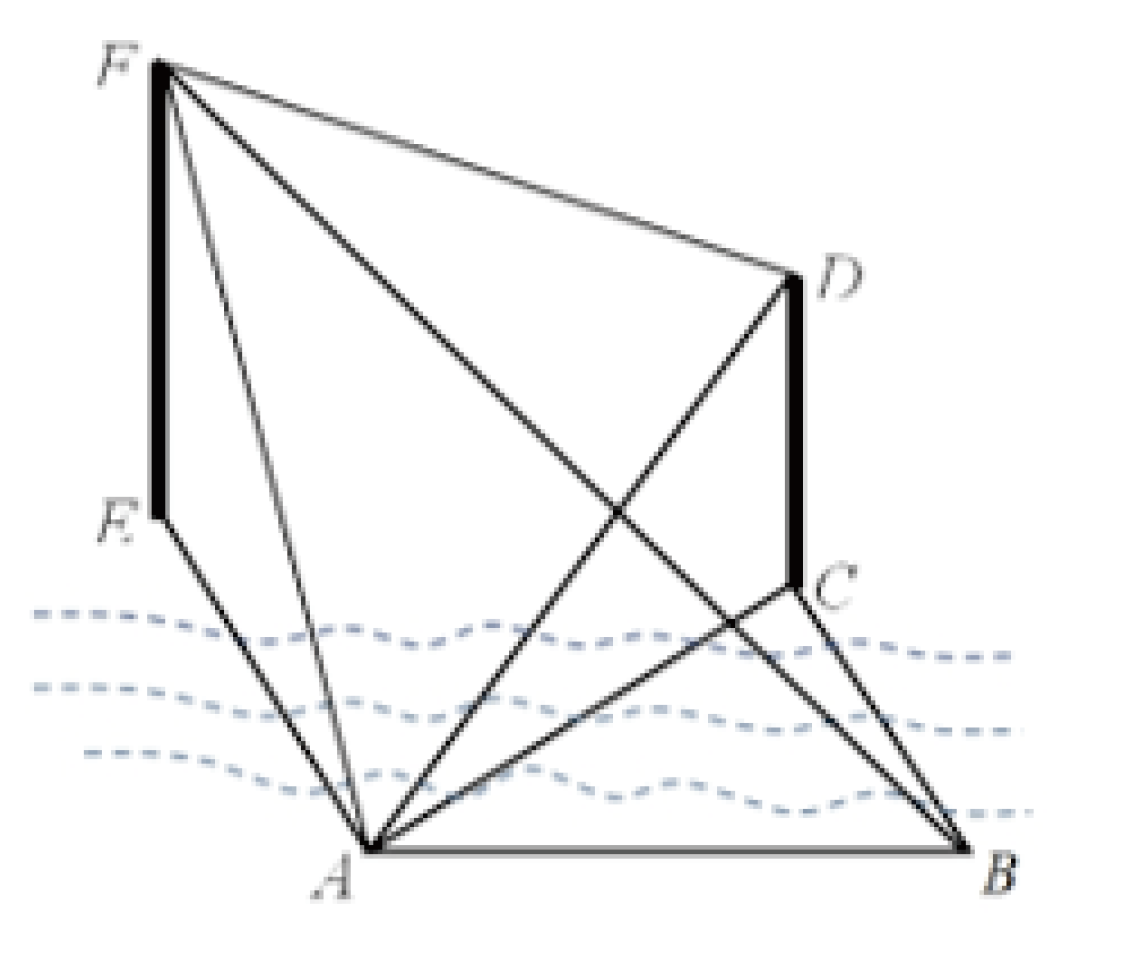
\includegraphics[scale = 0.3]{Q18.png}
		\]

		\begin{enumerate}[label = \calword{(\arabic*)}]
			\item 请你根据小明的测量数据求出塔\(CD\)高度; \answord{\(50 \sqrt{2}\)米}.

				\answord{解析.} 在\(\triangle ABC\)中, \(\angle ACB = 180\degree - \angle CAB - \angle CBA = 180\degree - 75\degree - 60\degree = 45\degree\). 由正弦定理, 有

				\[
					\frac{AC}{\sin \angle CBA} = \frac{AB}{\sin \angle ACB},
				\]

				所以有\(AC = \dfrac{100 \times \sin 60\degree}{\sin 45\degree} = 50 \sqrt{6}\)米.

				又有题意有, \(DC \bot AC, \angle DAC = 30\degree\), 所以有\(\ansmath{CD} = AC \cdot \tan \angle DAC = 50 \sqrt{6} \times 30\degree \ansmath{= 50\sqrt{2}}\)\answord{米}.

			\item 在完成\calword{(1)}的任务后, 小明想要计算两塔顶之间的距离\(DF\). 在测得\(\angle BAE = 90\degree\)之后, 小明并且准备再测量两个角的大小, 并为此准备了如下三个方案:

				\begin{multicols}{2}
					\begin{enumerate}[label = \calword{方案\arabic*.}]
						\item 测量\(\angle ABF\)和\(\angle DAF\);
						\item 测量\(\angle ABE\)和\(\angle EAF\);
						\item 测量\(\angle ABE\)和\(\angle ECF\);
						\item 测量\(\angle ABF\)和\(\angle AFB\).
					\end{enumerate}
				\end{multicols}

				请问: 小明的备选方案中有哪些是可行的? 写出所有可行方案的序号. \answord{(1), (2).}

				\answord{解析.} 解三角形.

				\calword{方案 3, 4} 不可行. 角的顶点\(C, F\)位于河对岸, 题干描述中提到了 "不渡过河的条件下".

				\calword{方案 1} 可行. 已知\(\angle ABF, \angle DAF\), 则\(\Rt \triangle ABF\)可解, \(\Rt \triangle ADF\)可解.

				\calword{方案 2} 可行. 已知\(\angle ABE, \angle EAF\), 则\(\Rt \triangle ABE\)可解, 则\(\triangle EAC\)可解, \(\triangle AEF\)可解, 在\(EF\)上截取\(EG=CD\), 有 \(\triangle DGF\)可解.

			\item 选择\calword{(2)}中的一种方案, 并结合以下数据, 计算出两塔顶\(DF\)之间的距离, 精确到米.

				\(\angle ABF = 58.0\degree, \angle ABE = 50.2\degree, \angle DAF = 16.7\degree, \angle EAF = 41.5\degree, \angle ECF = 53.8\degree, \angle AFB = 32.0\degree.\)

				\answord{解析.} 解三角形.

				由\calword{(1)}有, \(AD = \dfrac{CD}{\sin 30\degree} = 100\sqrt{2}\)米.

				在\(\Rt \triangle ABF\)中, \(AF = AB \cdot \tan \angle ABF = 100 \cdot \tan 58.0 \degree = 160.03\)米,

				在\(\triangle ADF\)中, 由余弦定理有

				\begin{align*}
					DF &= \sqrt{AD^2 + AF^2 - 2 AD \cdot AF \cdot \cos \angle DAF}\\
					   &= \sqrt{\left(100 \sqrt{2}\right)^2 + 160.03^2 - 2 \times 100\sqrt{2} \times 16 \times \cos 16.7 \degree}\\
					   &\approx 47,
				\end{align*}

				故\answord{两塔顶\(DF\)之间的距离为\(47\)米}.

		\end{enumerate}

	\section{特别致谢}
		\refword{stOOrz\_zyz34.} 提供答案参考.

\end{document}